%(BEGIN_QUESTION)
% Copyright 2007, Tony R. Kuphaldt, released under the Creative Commons Attribution License (v 1.0)
% This means you may do almost anything with this work of mine, so long as you give me proper credit

Anta at denne prosessen er optimalt innstilt, med et måleområde fra 0$^{o}$ F til 100$^{o}$ F:

$$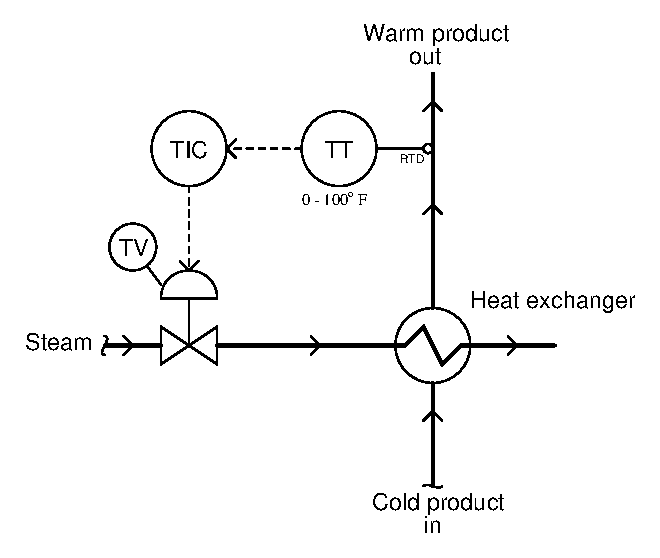
\includegraphics[width=15.5cm]{i01643x01.eps}$$

Deretter tas det en dag en beslutning om å områdesette temperaturtransmitteren (TT) på nytt for bedre oppløsning: 50$^{o}$ F til 70$^{o}$ F i stedet for 0$^{o}$ F til 100$^{o}$ F. Som resultat av denne områdeendringen begynner prosessen å oscillere rundt setpunkt i stedet for å holde seg stabil ved setpunkt, slik den gjorde tidligere.

\vskip 10pt

Forklar hvorfor denne områdeendringen gjorde prosesstyringen ustabil, og foreslå en løsning som gjenoppretter den tidligere reguleringskvaliteten.

\vfil

\underbar{file i01643}
\eject
%(END_QUESTION)





%(BEGIN_ANSWER)

Dette er et vurdert spørsmål -- ingen svar eller hint er gitt!

%(END_ANSWER)





%(BEGIN_NOTES)

Områdeendringen økte prosessforsterkningen effektivt med faktor fem. Med et transmitterområde som er 5 ganger smalere (nytt spenn er 20$^{o}$ F, fra gammelt spenn på 100$^{o}$ F), vil regulatoren se et prosessvariabelsignal (PV) som er 5 ganger mer følsomt for endringer i prosesstemperaturen enn før. For å hindre at regulatoren overreagerer på PV-endringer, må regulatorens aggressivitet reduseres tilsvarende med en faktor på 5.

\vskip 10pt

Når forsterkningen i en reguleringssløyfe endres som følge av endret transmitterspenn, endret ventil-C$_{v}$, eller et annet forsterkningsendrende forhold i prosessen, må {\it alle} regulatorledd endres omvendt (P, I {\it og} D), ikke bare ``P''-leddet.

En regulator som bruker enten {\it ideal}- eller {\it serie}-ligningen vil være enklere å stille inn på nytt ved endringer i total sløyfeforsterkning enn en regulator basert på {\it parallell}-ligningen, fordi én innstillingskonstant (K$_{c}$) påvirker alle tre reguleringsleddene proporsjonalt. Med {\it parallell}-ligningen må alle tre innstillingskonstanter justeres for å oppnå samme reguleringskvalitet som før.

Det er ingen forskjell i hvor enkelt det er å stille inn på nytt mellom {\it ideal}- og {\it serie}-ligningen i et scenario som dette.

%INDEX% Control, proportional + integral + derivative: ideal (ISA) equation
%INDEX% Control, proportional + integral + derivative: parallel equation
%INDEX% Control, proportional + integral + derivative: series equation
%INDEX% Process: heat exchanger temperature control (generic)

%(END_NOTES)
